\chapter{ Sprint0: Analyse Et  spécification des besoins}
\section*{Introduction}
Avant d'entamer le développement proprement dit de l'application, il est essentiel de passer par une phase d'analyse approfondie afin de bien cerner les besoins fonctionnels et non fonctionnels du système à concevoir. Cette étape, souvent désignée comme \textbf{Sprint 0} dans les méthodologies agiles, joue un rôle fondamental dans la réussite du projet, en permettant de clarifier les objectifs, d’identifier les acteurs concernés et de formaliser les exigences.

Dans ce chapitre, nous présentons les différents types de besoins identifiés à partir des attentes des utilisateurs finaux et des contraintes opérationnelles. Nous abordons également l’identification des parties prenantes, les cas d’usage principaux, ainsi que les spécifications techniques et fonctionnelles nécessaires à la mise en œuvre de la solution.

L'objectif principal de ce sprint préparatoire est d'établir une base solide et structurée sur laquelle les itérations de développement futures pourront s’appuyer de manière cohérente et efficace. \\

\section{Identification des acteurs }
Dans cette section, nous identifions les différents acteurs intervenant dans le système, qu’ils soient utilisateurs finaux ou parties techniques. Chacun de ces acteurs interagit avec le système selon des rôles et des responsabilités spécifiques. Leur identification permet de définir les cas d’usage associés à chaque profil et de modéliser les interactions attendues.
 \\

\subsection*{1. Client}
\begin{itemize}
  \item \textbf{Description} : Personne physique ou morale souhaitant réserver un service à travers la plateforme.
  \item \textbf{Interactions principales} :
    \begin{itemize}
        \item Interaction avec le chatbot pour décrire le besoin.
        \item Validation de la demande et réception d’un récapitulatif.
        \item Consultation du profil du helper et échange via messagerie.
        \item Réception de facture à la fin de la prestation.
    \end{itemize}
\end{itemize}

\subsection*{2. Prestataire de service }
\begin{itemize}
  \item \textbf{Description} : Travailleur indépendant ou employé référencé sur la plateforme, chargé d’exécuter les prestations demandées par les clients.
  \item \textbf{Interactions principales} :
    \begin{itemize}
        \item Consulter la liste des demandes de services disponibles qui correspondent à son domaine de compétence.
        \item Manifester son intérêt pour une demande spécifique afin d’en proposer la prise en charge.
        \item Communiquer avec le client par le biais de la messagerie intégrée pour clarifier les détails de l’intervention.
        \item Suivre l’historique de ses prestations et consulter ses gains réalisés.
        \item Accéder à ses documents de facturation générés automatiquement après la réalisation des missions.
        \item Consulter son calendrier personnel pour planifier ses disponibilités et interventions.
    \end{itemize}
\end{itemize}

\subsection*{3. Administrateur d’entité (Office Admin)}
\begin{itemize}
  \item \textbf{Description} : Responsable local de la gestion de l’entité cliente (par exemple une franchise ou une entreprise abonnée à la solution).
  \item \textbf{Interactions principales} :
    \begin{itemize}
        \item Validation des comptes helpers.
        \item Gestion des utilisateurs, des ressources et des services.
        \item Consultation des ordres en cours et des historiques.
        \item Suivi des paiements et des performances opérationnelles.
    \end{itemize}
\end{itemize}

\subsection*{4. Chatbot}
\begin{itemize}
  \item \textbf{Description} : Agent conversationnel intelligent chargé de guider l’utilisateur (client) dans la description de ses besoins.
  \item \textbf{Interactions principales} :
    \begin{itemize}
        \item Dialogue interactif avec le client.
        \item Collecte d’informations pour créer un ordre.
        \item Validation des données saisies.
    \end{itemize}
\end{itemize}
\section{Besoins fonctionnels}

Les besoins fonctionnels représentent les fonctionnalités essentielles que le système doit offrir afin de répondre aux attentes des différents utilisateurs identifiés. Ils sont classés selon les principales catégories d’interaction avec la plateforme.

\subsection*{1. Gestion des clients}
\begin{itemize}
    \item Création et gestion d’un compte client.
    \item Accès à une interface de demande de service via un agent conversationnel (chatbot).
    \item Suivi des demandes en cours et passées.
    \item Consultation des profils des prestataires qui ont exprimer leurs intérêts .
    \item Communication avec le prestataire avant ou après l’acceptation d’une demande.
    \item Réception automatique de la facture après la réalisation du service.
\end{itemize}

\subsection*{2. Gestion des prestataires}
\begin{itemize}
    \item Inscription et soumission des informations personnelles et professionnelles.
    \item Accès à un tableau de bord regroupant les demandes disponibles.
    \item Possibilité de manifester un intérêt pour un ordre de mission.
    \item Consultation de l’historique de travail et du montant des revenus générés.
    \item Visualisation des factures associées à ses interventions.
    \item Consultation du calendrier de travail.
    \item Communication avec les clients via une messagerie intégrée.
\end{itemize}

\subsection*{3. Gestion des ordres de mission}
\begin{itemize}
    \item Génération automatique d’un ordre à partir d’un échange avec le chatbot.
    \item Affectation de l’ordre aux prestataires concernés selon leur profil et disponibilité.
    \item Suivi des étapes de l’intervention (confirmation, en route, démarrage, fin).
    \item Clôture automatique de l’ordre et déclenchement de la facturation.
\end{itemize}

\subsection*{4. Administration de la plateforme}
\begin{itemize}
    \item Validation et activation des comptes des prestataires inscrits.
    \item Suivi en temps réel de l’ensemble des ordres de mission et consultation de leur historique.
    \item Supervision globale de l’activité des utilisateurs (clients, prestataires).
    \item Gestion des types de services offerts par entité (création, modification, désactivation).
    \item Suivi des paiements effectués et des performances opérationnelles (durée moyenne des interventions, taux de satisfaction, volume d’activité, etc.).
    \item Gestion des rôles, des droits d’accès et des paramètres globaux de la plateforme.
\end{itemize}


\section{Besoins non fonctionnels}

Les besoins non fonctionnels définissent les contraintes de qualité, de performance et de sécurité que le système doit respecter pour garantir une expérience utilisateur optimale, une évolutivité correcte et une exploitation fiable.

\subsection*{1. Performance}
\begin{itemize}
    \item Le temps de réponse de l’interface ne doit pas dépasser 2 secondes pour toute action courante (consultation, navigation, envoi de message, etc.).
    \item Le système doit pouvoir traiter simultanément plusieurs centaines d’utilisateurs sans dégradation notable des performances.
\end{itemize}

\subsection*{2. Sécurité}
\begin{itemize}
    \item Toutes les communications doivent être chiffrées via HTTPS.
    \item L’authentification doit être sécurisée et basée sur des mots de passe robustes.
    \item L’accès aux données doit être strictement contrôlé en fonction des rôles (client, prestataire, administrateur, etc.).

\end{itemize}

\subsection*{3. Fiabilité}
\begin{itemize}
    \item Le système doit garantir une disponibilité supérieure à 99.5\% en période de production.
    \item Des mécanismes de sauvegarde régulière des données doivent être mis en place pour assurer la continuité de service.
\end{itemize}

\subsection*{4. Accessibilité et compatibilité}
\begin{itemize}
    \item L’application doit être accessible depuis tout navigateur moderne (Chrome, Firefox, Safari, Edge).
    \item L’interface doit être responsive, c’est-à-dire parfaitement adaptée à une utilisation sur ordinateur, tablette et smartphone.
\end{itemize}

\subsection*{5. Maintenabilité et évolutivité}
\begin{itemize}
    \item L’architecture logicielle doit permettre l’ajout de nouvelles fonctionnalités sans remettre en cause les composants existants.
    \item Le code doit être structuré, documenté et conforme aux bonnes pratiques de développement (normes PEP8 pour Python, modularité...).
\end{itemize}

\subsection*{6. Ergonomie}
\begin{itemize}
    \item L’interface utilisateur doit être simple, intuitive et accessible à un public non technique.
    \item Le chatbot doit proposer un langage naturel fluide, compréhensible et adapté aux requêtes des utilisateurs.
\end{itemize}

\section{Spécification Des Besoins}

La spécification des besoins a pour objectif de formaliser les attentes fonctionnelles du système sous forme de cas d’utilisation, en tenant compte des différents acteurs identifiés. Elle constitue une base essentielle pour la conception, le développement et la validation de l’application.

\subsection{Définition}

Un \textbf{cas d’utilisation} (ou \textit{use case}) représente une interaction typique entre un utilisateur (acteur) et le système dans le but d’atteindre un objectif précis. Chaque cas d’utilisation décrit un scénario métier ou fonctionnel, sans entrer dans les détails techniques d’implémentation.

Les cas d’utilisation permettent :
\begin{itemize}
    \item D’identifier clairement les fonctionnalités attendues par chaque acteur.
    \item De structurer les interactions possibles avec le système.
    \item De servir de support à la modélisation UML pour les phases suivantes de conception.
\end{itemize}

\section{Spécification des besoins}

\subsection{Diagramme de cas d’utilisation}

\subsubsection*{Définition}

Les diagrammes de cas d’utilisation sont un outil fondamental en analyse des systèmes. Ils offrent une représentation structurée des fonctionnalités d’un système du point de vue de ses utilisateurs (\textit{acteurs}). Ces diagrammes permettent de capturer le \og quoi \fg{} du système, en décrivant les actions que les utilisateurs peuvent effectuer pour atteindre des objectifs spécifiques, plutôt que les détails techniques du \og comment \fg{} ces fonctionnalités sont mises en œuvre.

\paragraph*{Acteurs :}
Les acteurs représentent des entités externes (individus, systèmes tiers ou tout autre élément extérieur) qui interagissent avec le système pour accomplir un objectif donné. Ils sont généralement représentés par des figures en forme de bâtonnets ou des pictogrammes.

\paragraph*{Cas d’utilisation :}
Les cas d’utilisation représentent les services ou fonctionnalités proposés par le système. Ils sont illustrés sous forme d’ellipses et décrivent une suite d’actions entreprises par un acteur pour atteindre un but précis.

\subsubsection*{Diagramme de cas d’utilisation global}

Le diagramme de cas d’utilisation global suivant présente les principales interactions entre les différents acteurs du système (client, prestataire, administrateur, etc.) et les fonctionnalités proposées par la plateforme.

\begin{figure}[H]
    \centering
    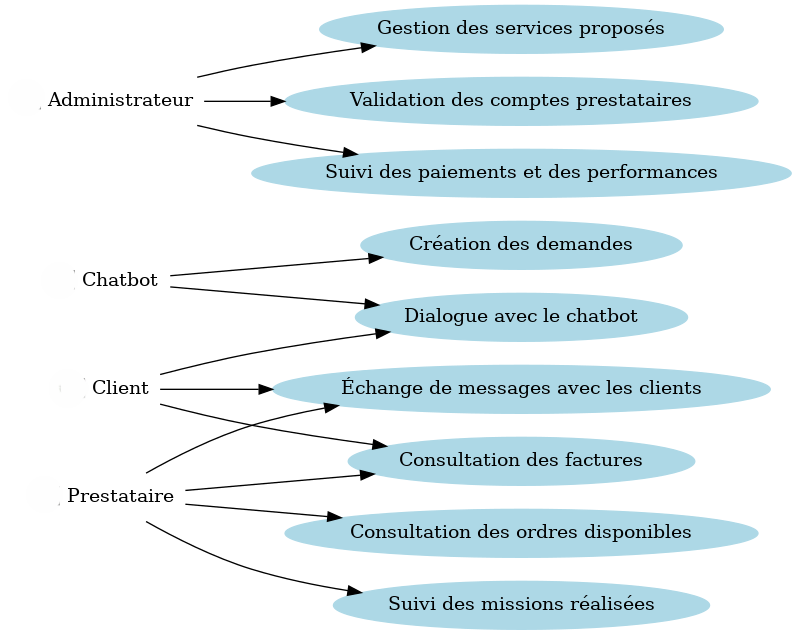
\includegraphics[width=0.9\textwidth]{figures/use_case_global.png} % Remplacer par le nom réel du fichier
    \caption{Diagramme de cas d’utilisation global du système}
    \label{fig:usecase_global}
\end{figure}
\medskip

\noindent
Ce diagramme illustre les différentes actions possibles selon les rôles :
\begin{itemize}
    \item \textbf{Administrateur} : peut gérer les services proposés, valider les comptes prestataires, et assurer le suivi des paiements ainsi que des performances opérationnelles.
    \item \textbf{Prestataire} : peut consulter les ordres disponibles, suivre l’historique de ses missions, consulter ses factures et échanger avec les clients via la messagerie.
    \item \textbf{Client} : peut dialoguer avec le chatbot, recevoir les factures et communiquer avec le prestataire pour organiser la mission.
    \item \textbf{Chatbot} : est chargé d’interagir avec le client afin de collecter les informations nécessaires à la création automatique d’une demande.
\end{itemize}
\section{Architecture du système}
\subsection{Architecture physique}

L’architecture physique de notre application repose sur une architecture classique à trois niveaux (3-tiers), comme illustré dans la figure suivante :

\begin{figure}[H]
    \centering
    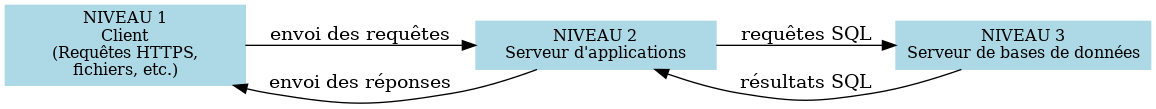
\includegraphics[width=0.75\textwidth]{figures/architecture_physique.png}
    \caption{Architecture physique à trois niveaux}
    \label{fig:architecture_physique}
\end{figure}

L’architecture représentée dans la figure \ref{fig:architecture_physique} se divise en trois niveaux principaux :

\begin{enumerate}
    \item \textbf{Niveau 1 : Client}
    \begin{itemize}
        \item Ce niveau représente l’utilisateur final accédant à l’application via un navigateur web.
        \item Il envoie des requêtes HTTPS à travers l’interface développée avec Angular (frontend SPA).
        \item Il reçoit les réponses en retour après traitement.
    \end{itemize}
    
    \item \textbf{Niveau 2 : Serveur d'applications}
    \begin{itemize}
        \item Il constitue le cœur logique de l’application et est construit avec le framework Django.
        \item Il gère la logique métier, l’authentification, la gestion des utilisateurs, la création des ordres, la facturation, etc.
        \item Ce serveur reçoit les requêtes du client, les traite, et communique avec la base de données via une API REST.
        \item Tous les composants sont conteneurisés avec Docker pour assurer la portabilité, l’isolation et la scalabilité du système.
    \end{itemize}
    
    \item \textbf{Niveau 3 : Serveur de bases de données}
    \begin{itemize}
        \item Ce niveau est assuré par PostgreSQL, également déployé dans un conteneur Docker.
        \item Il stocke toutes les données métier, y compris les entités, les utilisateurs, les ordres, les prestations, les factures, etc.
        \item Il répond aux requêtes SQL envoyées par le serveur d’applications et renvoie les données nécessaires à l’exécution des traitements.
    \end{itemize}
\end{enumerate}

\medskip

Grâce à l'utilisation de Docker, les trois niveaux de cette architecture sont déployés dans des conteneurs distincts, facilitant ainsi le déploiement, la maintenance et l’évolution du système. Cette approche garantit également une meilleure gestion des dépendances et une indépendance vis-à-vis de l’infrastructure matérielle sous-jacente.

\subsection{Architecture logique}
\subsubsection{Architecture Django}
L’architecture logique de l’application repose sur le paradigme \textbf{MVT (Model-View-Template)} proposé par le framework Django. Cette architecture organise le développement en trois composants principaux, chacun assumant une responsabilité bien définie.

\begin{figure}[H]
    \centering
    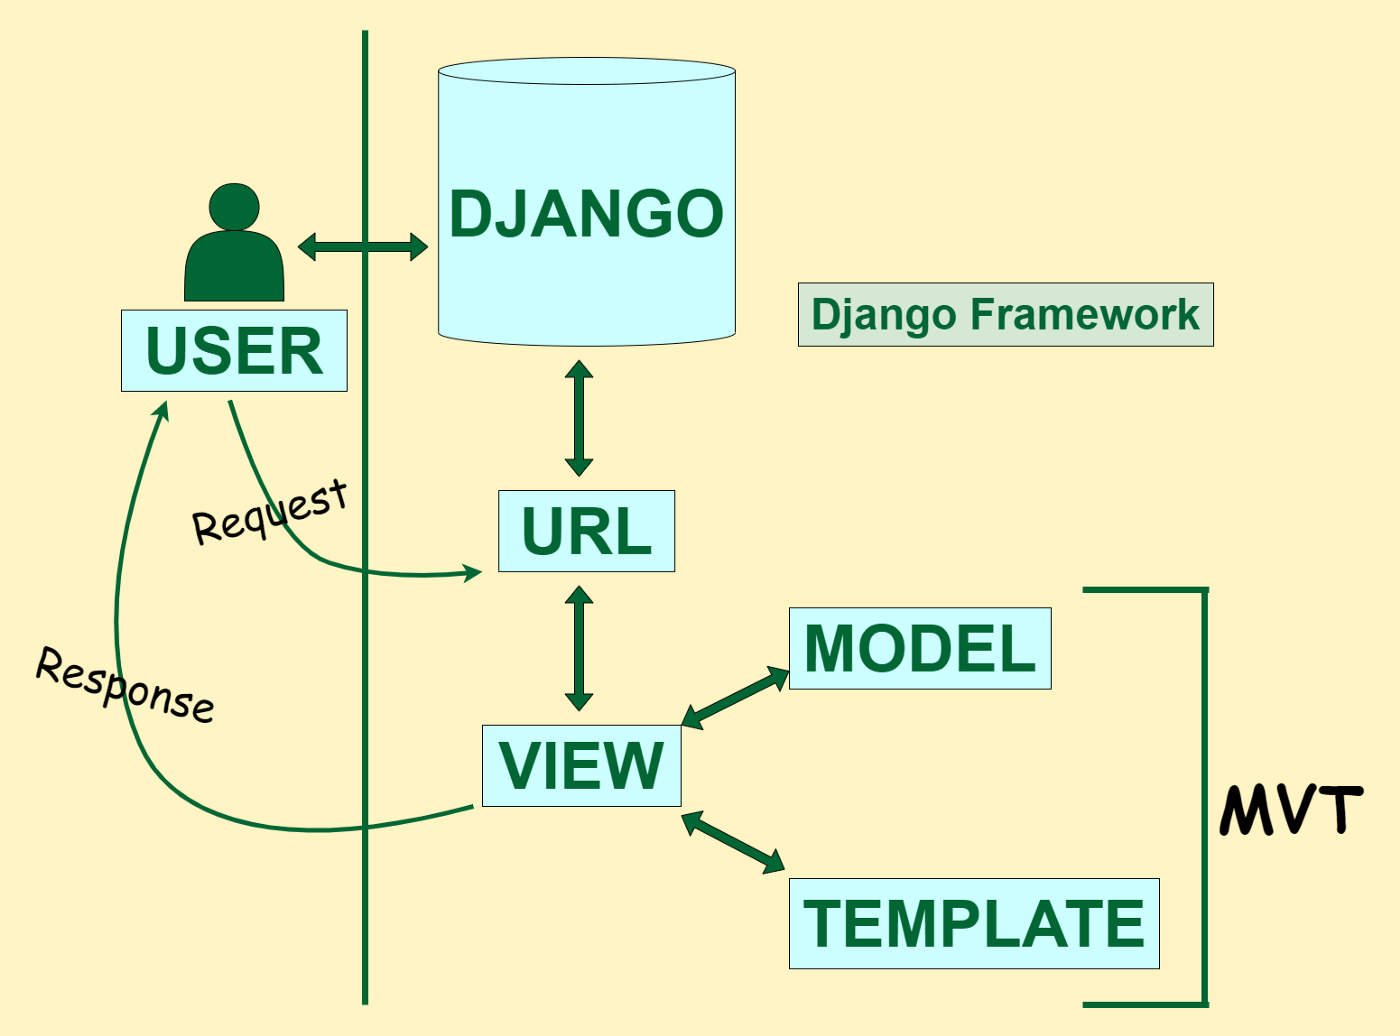
\includegraphics[width=0.9\textwidth]{figures/django architecture.png}
    \caption{Architecture Django MVT}
    \label{fig:architecture_mvt}
\end{figure}

L’architecture illustrée dans la figure \ref{fig:architecture_mvt} se structure comme suit :

\begin{enumerate}
    \item \textbf{Model (Couche base de données)} :
    \begin{itemize}
        \item Gère les données et les interactions avec la base de données relationnelle.
        \item Permet d’effectuer des opérations CRUD (\textit{Create, Read, Update, Delete}).
        \item Utilise des objets Python (modèles) pour représenter les tables et les enregistrements.
    \end{itemize}
    
    \item \textbf{View (Organisation et préparation des données)} :
    \begin{itemize}
        \item Traite les requêtes HTTP reçues depuis le navigateur.
        \item Récupère les données via les modèles, applique la logique métier, et transmet les résultats au Template.
        \item Ne génère pas directement l’interface utilisateur.
    \end{itemize}
    
    \item \textbf{Template (Couche présentation)} :
    \begin{itemize}
        \item Gère l’affichage de l’interface utilisateur (UI).
        \item Utilise HTML, CSS et JavaScript pour structurer et styliser l'affichage.
        \item Intègre dynamiquement les données transmises par la View.
    \end{itemize}
    
    \item \textbf{Utilisateur et Navigateur} :
    \begin{itemize}
        \item L’utilisateur interagit avec l’application via un navigateur.
        \item Le navigateur envoie des requêtes HTTP au serveur Django, qui renvoie les réponses après traitement.
    \end{itemize}
\end{enumerate}
\medskip

\noindent
Cette architecture MVT est similaire au modèle MVC (Model-View-Controller), mais diffère légèrement en ce que Django traite automatiquement certaines fonctions du contrôleur, en intégrant les templates dans la structure. 
\subsubsection{Architecture Angular}

L’architecture Angular repose sur une approche modulaire et basée sur des composants pour le développement d’applications web dynamiques et interactives. Elle permet de structurer l’interface utilisateur de manière claire, évolutive et réutilisable.

\begin{figure}[H]
    \centering
    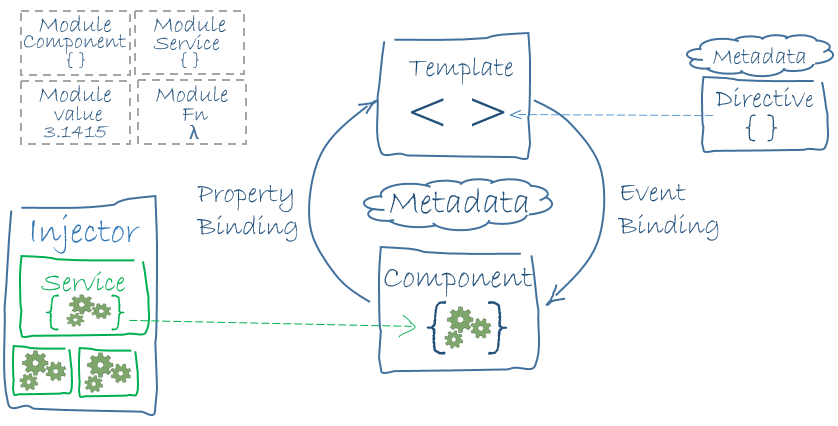
\includegraphics[width=0.8\textwidth]{figures/angular architecture.png}
    \caption{Architecture d’Angular}
    \label{fig:architecture_angular}
\end{figure}

Les éléments clés de cette architecture sont les suivants :

\begin{enumerate}
    \item \textbf{Template} :
    \begin{itemize}
        \item Représente la couche de présentation.
        \item Définit l’interface utilisateur à l’aide de balises HTML et de directives Angular.
        \item Permet l’intégration de données dynamiques provenant des composants grâce au \textit{Property Binding} (liaison de propriété) et au \textit{Event Binding} (liaison d’événements).
    \end{itemize}

    \item \textbf{Component} :
    \begin{itemize}
        \item Une unité principale contenant la logique métier liée à une partie spécifique de l’interface utilisateur.
        \item Chaque composant est associé à un template et est responsable de gérer les données et les événements interactifs de ce template.
    \end{itemize}

    \item \textbf{Metadata} :
    \begin{itemize}
        \item Fournit des informations supplémentaires sur une classe Angular (par exemple, si une classe représente un composant ou un service).
        \item Sert à lier un composant à son template, et à configurer les comportements des directives ou des services.
    \end{itemize}

    \item \textbf{Injector et Services} :
    \begin{itemize}
        \item Angular utilise un système d’injection de dépendances (\textit{Dependency Injection}) via un \textit{Injector}, qui permet de fournir des services aux composants.
        \item Les services contiennent des logiques réutilisables, telles que la gestion des données ou des appels à une API, et peuvent être partagés entre plusieurs composants.
    \end{itemize}

    \item \textbf{Property Binding et Event Binding} :
    \begin{itemize}
        \item \textbf{Property Binding} : permet de transmettre des données d’un composant vers son template (flux unidirectionnel).
        \item \textbf{Event Binding} : gère les interactions utilisateur (par exemple, clics) en reliant des événements du template au code du composant.
    \end{itemize}

    \item \textbf{Directives} :
    \begin{itemize}
        \item Ce sont des éléments personnalisés permettant de manipuler le DOM ou d’appliquer des comportements dynamiques à des éléments HTML.
    \end{itemize}
\end{enumerate}

\medskip

\noindent
En résumé, l’architecture Angular favorise la \textbf{modularité}, la \textbf{réutilisabilité} et une \textbf{séparation claire des responsabilités}, ce qui en fait un choix populaire pour le développement d’applications web modernes.

\section*{Conclusion}

Ce premier sprint a permis d'établir une vision claire et partagée du système à concevoir. Grâce à l'analyse des besoins fonctionnels et non fonctionnels, à l’identification rigoureuse des acteurs et à la formalisation des cas d’usage, nous avons posé les fondations solides pour le développement de l’application.

La documentation produite à ce stade constitue un référentiel de référence pour les équipes techniques et fonctionnelles tout au long du projet. Elle garantit une compréhension commune des attentes utilisateurs, des objectifs métiers et des contraintes techniques.

Ce travail préparatoire, bien que non directement productif en termes de livrables logiciels, est indispensable pour assurer la cohérence, la qualité et la maintenabilité du produit final. Il ouvre la voie à un développement agile plus efficace et plus ciblé dès le Sprint 1.
